\section{Attitude Controller}\label{sec:AttitudeControllerDesign}
The attitude controller constitutes an inner loop which receives references for the roll and pitch, from the outer loop which is the $x_{\mathrm{I}}$ and $y_{\mathrm{I}}$ translational controller. As it is decided only to move the drone in one inertial axis at a time, the plus configuration explained in \autoref{chap:Model} \fxnote{Ensure that it matches what is written in the model section}, the yaw reference is always set to zero.\\ The angular response of the quadcopter constitutes a coupled behavior, as all the three Euler angles ($\phi$, $\theta$ and $\psi$) are affected by the same four motor velocities, see \autoref{fig:ControlHeadDiagram}. This makes it harder to utilize independent controllers for each angle. A state space approach is therefore utilized, as this method is less complicated when the system to be controlled has multiple input and multiple sensed outputs \cite{MultipleInputandoutput}.

The system behavior is represented by means of the linearized model equations. These linearized equations can be represented in state variable form, shown in \autoref{xDotLinear} and \ref{yLinear}.
%
\begin{flalign}
	\vec{\dot{x}}(t)&=\vec{A} \  \vec{x}(t) + \vec{B} \  \vec{u}(t)
	\label{xDotLinear} 
\end{flalign}
\begin{flalign}
	\vec{y}(t)&=\vec{C} \  \vec{x}(t) + \vec{D} \  \vec{u}(t)
	\label{yLinear} 
\end{flalign}
%
\begin{where}	
	\va{\vec{x}}{are the states of the system}{}
    \va{\vec{A}}{is the system matrix}{}
    \va{\vec{B}}{is the input matrix}{}
    \va{\vec{C}}{is the output matrix}{}
    \va{\vec{D}}{is the direct transmission term}{}
\end{where}

A block diagram of the state space description can be seen in \autoref{SSBlocks}.
%
\begin{figure}[H]
	\begin{tikzpicture}[ auto,
                       thick,                         %<--setting line style
                       node distance=1.5cm,             %<--setting default node distance
                       scale=1,                     %<--|these two scale the whole thing
                       every node/.style={scale=1}, %<  |(always change both)
                       >=triangle 45 ]                %<--sets the arrowtype
    
    \draw%-----------------------------------------------------------------------------------------
    	%Drawing Input/Output:
    	node[shape=coordinate][](input1) at (0,0){}
    	node[shape=coordinate][](output1) at (9.5,0){}
     	%Drawing the Equation Blocks:   	
      	node(A) at (4.5,-1.5) [block] {A} 
     	node(B) at (1.5,0) [block] {B}
     	node(C) at (6.5,0) [block] {C}
      	node(D) at (4.5,1.5) [block] {D}  
	    node(int) at (4.5,0) [block] {\si{\int}}  
    	%Drawing the Sumation Blocks:	    	 	
    	node(sum1) [sum, right of = B] {\si{\sum}}
    	node(sum2) [sum, right of = C] {\si{\sum}}
    	%Drawing the Feedback/Feedforward Nodes:    	
    	node[shape=coordinate][](FeedforwardNode) at (0.75,0){}
    	node[shape=coordinate][](FeedbackNode) at (5.5,0){}  	
    	     
    ;%---------------------------------------------------------------------------------------------
   
    %Joining the Blocks
  	\draw[->](input1) -- node {u}(B);
  	\draw[->](B) -- node {}(sum1);
  	\draw[->](sum1) -- node {\si{\dot x}}(int);  	
  	\draw[->](int) -- node {x}(C);
  	\draw[->](C) -- node {}(sum2);  	
  	\draw[->](sum2) -- node {y}(output1);
  	
  	\draw[->](FeedforwardNode) |- node{} (D);
  	\draw[->](D) -| node{} (sum2);

  	\draw[-] (FeedbackNode) |- (A);
  	\draw[->] (A)   -| (sum1);

    %Drawing node(s) with \textbullet
    \draw%--------------------------------------------------------------
      node at (input1)  [shift={(-0.08, -0.02 )}] {\large \textbullet}
    	% node at (output1) [shift={( 0.008, -0.02 )}] {\textbullet}
    ;%------------------------------------------------------------------
  \end{tikzpicture}
	\centering
	\caption{Block diagram of the state space representation of the system.}
	\label{SSBlocks}
\end{figure}\vspace{-18pt}
%
For an nth-order system the states of the system, $\vec{x}$, is a vector containing n elements. Thus the $\vec{x}$ vector contains six elements, as there are three attitude equations each with an order of two. The equations are found in \autoref{sec:CombinedModel}. Typically for a mechanical system the states are the velocities and the position of the system, as Newton's law is utilized \cite{Stateschosen}. This corresponds with the three attitude equations, as Newton's law is utilized yielding an equation with angular acceleration included. The states are therefore the three angular velocities and the three angles. \\
The size of the input vector, $\vec{u}$, is $m \times 1$ vector, where m is the number of inputs. The inputs are the four motor velocities. The output, $\vec{y}$, contains the three angles, $\phi$, $\theta$ and $\psi$. From now on, the variables in the equations are represented without the symbol $\Delta$, as to avoid excessive symbol notation, even though they refer to changes around the linearization point. The generated vectors can be seen in \autoref{uVector}.\\
\begin{minipage}{0.32\linewidth}
	\begin{flalign}
		\vec{x}(t) = 
		\begin{bmatrix}
			\phi \\
			\theta \\ 
			\psi \\
			\dot{\phi} \\
			\dot{\theta} \\
			\dot{\psi} \\
		\end{bmatrix}	\nonumber
		\label{xVector}
	\end{flalign}  
\end{minipage}\hfill
%\hspace{0.03\linewidth}
\begin{minipage}{0.32\linewidth}
	\begin{flalign}
		\vec{y}(t) = 
		\begin{bmatrix}
			\phi \\
			\theta \\ 
			\psi \\
		\end{bmatrix}	\nonumber
		\label{yVector}
	\end{flalign}
\end{minipage}\hfill
%\hspace{0.03\linewidth}
\begin{minipage}{0.32\linewidth}
	\begin{flalign}
		\vec{u}(t)= 
		\begin{bmatrix}
			\omega_1 \\
			\omega_2 \\
			\omega_3 \\
			\omega_4 \\
		\end{bmatrix}\textsl{}
		\label{uVector}
	\end{flalign}
\end{minipage}\hfill
\\
The specific matrices for the description of the angular behavior are obtained from the linearized equations of the system (\autoref{eqAngleLin1} and \ref{eqAngleLin2}). The size of the input matrix, $\vec{B}$, is $n \times m$, where n is the order of the system and m is the number of inputs. The size of the system matrix, $\vec{A}$, is an $n \times n$ and the output matrix, $\vec{C}$, is an $1 \times n$ matrix. The $\vec{C}$ matrix contains the states which are measured, this is decided to be the three angles. As the Vicon system measures the attitude of the quadcopter, and it is desired to have the reference for the attitude controller to be roll and pitch, see \autoref{fig:ControlHeadDiagram}. The matrices generated from the linear attitude equations are showed embedded in the state space representation in \autoref{xDotSS} and \autoref{ySS}.
%
\begin{flalign}   \label{xDotSS}
	\vec{\dot{x}}(t) &=
	\begin{bmatrix}
		\ 0 & 0 & 0 & 1 & 0 & 0     \ \ \ \\ 
		\ 0 & 0 & 0 & 0 & 1 & 0     \ \ \ \\ 
		\ 0 & 0 & 0 & 0 & 0 & 1     \ \ \ \\
		\ 0 & 0 & 0 & 0 & 0 & 0     \ \ \ \\ 
		\ 0 & 0 & 0 & 0 & 0 & 0     \ \ \ \\ 
		\ 0 & 0 & 0 & 0 & 0 & 0     \ \ \ 		
	\end{bmatrix}
	\vec{x}(t) +
	\begin{bmatrix}
		\ 0 & 0 & 0 & 0      \ \ \ \\ 
		\ 0 & 0 & 0 & 0      \ \ \ \\ 
		\ 0 & 0 & 0 & 0      \ \ \ \\
		\ 0 & \si{-\frac{2 \  k_{th} \  L \  \overline{\omega}_2}{J_x}} & 0 & \si{\frac{2 \  k_{th} \  L \  \overline{\omega}_4}{J_x}}      \ \ \ \\ 
		\ \si{\frac{2 \  k_{th} \  L \  \overline{\omega}_1}{J_y}} & 0 & \si{-\frac{2 \  k_{th} \  L \  \overline{\omega}_3}{J_y}} & 0      \ \ \ \\ 
		\ \frac{2 \  k_d \  {\overline{\omega}_1}}{J_z} & - \frac{2 \  k_d \  {\overline{\omega}_2}}{J_z} & \frac{2 \  k_d \  {\overline{\omega}_3}}{J_z} & - \frac{2 \  k_d \  {\overline{\omega}_4}}{J_z}      \ \ \ 		
	\end{bmatrix}
	\vec{u}(t)
\end{flalign}
\begin{flalign} \label{ySS}
	\vec{y}(t) &=	 
	\begin{bmatrix}
		\ 1 & 0 & 0 & 0 & 0 & 0     \ \ \ \\ 
		\ 0 & 1 & 0 & 0 & 0 & 0     \ \ \ \\ 
		\ 0 & 0 & 1 & 0 & 0 & 0     \ \ \ 		
	\end{bmatrix}
	\vec{x}(t)
\end{flalign}

Before deciding on controllers and if an observer should be utilized, it is advisable to check the controllability and observability of the system. For doing so, the matrices shown in \autoref{controlabilityandobservability} are used. \\
\begin{minipage}{0.45\linewidth}
\begin{flalign}
\vec{{\mathcal C}} = 
\begin{bmatrix}
\vec{B}&\vec{A}\vec{B}&\vec{A^2}\vec{B}&\vec{A^3}\vec{B}&\vec{A^4}\vec{B}&\vec{A^5}\vec{B} \\	
\end{bmatrix}\nonumber 
\end{flalign}
\end{minipage}\hfill
%\hspace{0.03\linewidth}
\begin{minipage}{0.45\linewidth}
\begin{flalign}
\vec{{\mathcal O}} = 
\begin{bmatrix}
\vec{C} \\
\vec{C}\vec{A} \\
\vec{C}\vec{A}^2 \\
\vec{C}\vec{A}^3 \\
\vec{C}\vec{A}^4 \\
\vec{C}\vec{A}^5 \\		
\end{bmatrix}					\label{controlabilityandobservability} 									
\end{flalign}
\end{minipage}\hfill

The rank of these matrices are six, that is, the number of states. This makes the system both controllable and observable. The precise value of the matrices can be seen in \autoref{app:matricesSS}. Note, if the measured states was the angular velocities and not the angles, the system would not have been observable, as the matrix would have a rank of three.

The dynamics of the system can be analyzed by looking at the system matrix $\vec{A}$. The eigenvalues of this matrix represent the location of the systems open loop poles. In this case, the system has six poles located in zero, which means that the system is marginally stable. In order to place those poles at a better location a state feedback is use. This is combined with an integral controller to be able to set a desired reference, different from zero, for the roll and pitch. 

%As the output is formed by the three angles, these are the only measured states in the system.
For doing the state feedback, the angular velocities are also needed even though they are not measured. The way of obtaining these is done by utilizing a reduced order observer. This is done even though the angular velocities could be estimated with a numerical differentiation procedure. The observer is more convenient in case of using on board sensors and by using it, that possibility is kept open. Furthermore from an learning perspective it is valuable.

This way of approaching the control of the system is simplified by the possibility of designing the state feedback, integral controller and the reduced order observer independently. This holds due to the separation principle.
The separation principle theorem states, an observer with gain $\vec{L}$ and a feedback with gain $\vec{F}$ results in 2n closed loop poles \cite{ObserverChristoffer}, where n is the number of states in the system. As a reduced order observer is utilized for estimating the angular velocities, only nine poles are created. 

A block diagram showing the system overview of the attitude controller is shown in \autoref{attitudecontrollerdiagram}. Here the state feedback, the integral control and the reduced order observer can be seen.
\begin{figure}[H]
	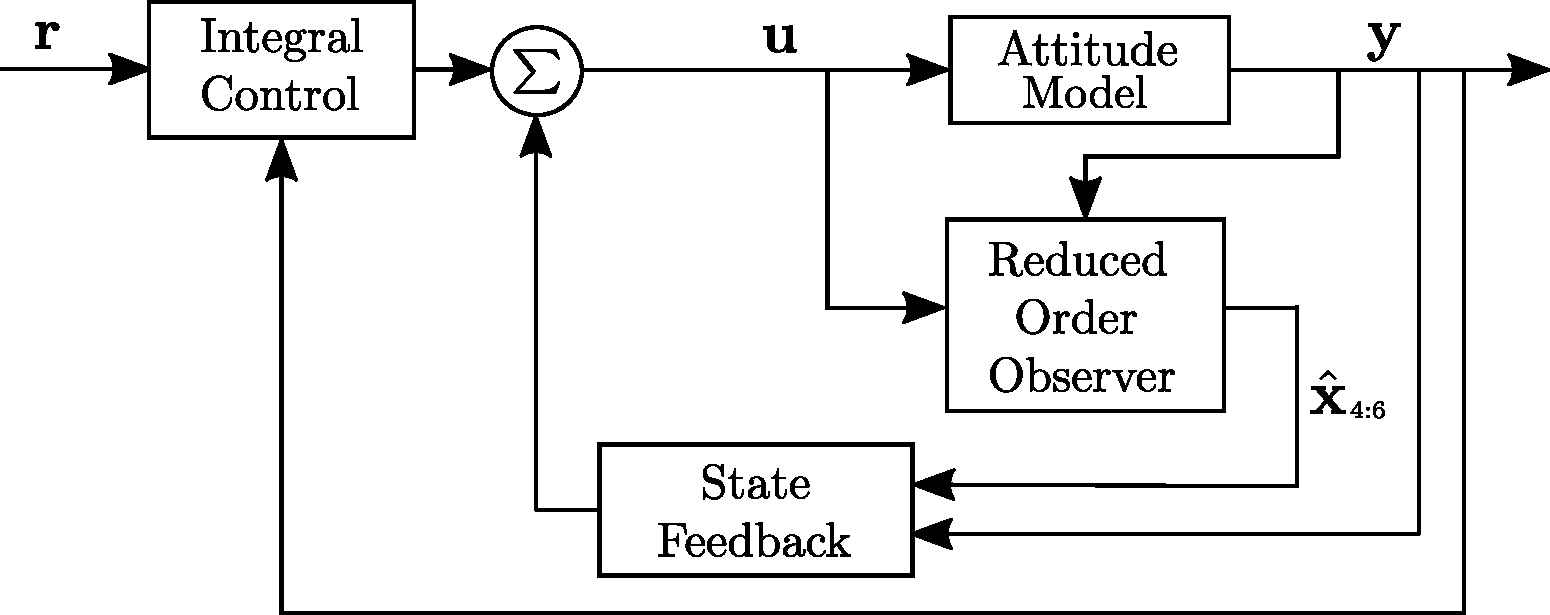
\includegraphics[scale=.5]{figures/AttitudeControlDiagram}
	\centering
	\caption{Control structure for the system, including the state feedback, the integral control and the reduced order observer.}
	\label{attitudecontrollerdiagram}
\end{figure}

In the following subsections, the state feedback with the integral control is designed and then the reduced order observer is designed.

%These show how the output and the states of the system evolve as a function of the current states values and the input applied to the system. \autoref{xDotDiffEq} and \autoref{yDiffEq} show the idea of state space representation.
%
%\begin{flalign}
%	\vec{\dot{x}}(t)&=f(\vec{x}(t),\vec{u}(t))
%	\label{xDotDiffEq} 
%\end{flalign}
%\begin{flalign}
%	\vec{y}(t)&=g(\vec{x}(t),\vec{u}(t)) 
%	\label{yDiffEq} 
%\end{flalign}
%